\section{Security Model}

The BioBankCloud environment deploys strong security features for concerns such as Confidentiality, Integrity and Non-repudiation ~\cite{BBCSEC} of data access. This includes authentication, authorization
, and auditing. The system allows defining different roles with different access privileges. In designing the system, we applied the Cloud Privacy Threat Modeling~\cite {CPTM} approach to identify the privacy requirements of processing sensitive biomedical data.



Figure \ref{fig:security} shows the different components of the employed security mechanisms. All BioBankCloud services are protected behind the firewall and only accessible through the secure interfaces over HTTPS Channels.


\begin{figure}[h]
\centering
\includegraphics[width=\textwidth]{./imgs/security.png}
% stack.eps: 0x0 pixel, 300dpi, 0.00x0.00 cm, bb=0 -1 805 312                                                                                                                                               
\caption{Security Architecture of the BiobankCloud}
\label{fig:security}
\end{figure}


\subsection{2-Factor Authentication}
 The authentication services map the person accessing the platform to a user identity. We provide two-factor authentication using smart mobile devices or Yubikey hardware tokens to support different groups of users.

\subsection {Access Control}
The accessc control component ensures authorized access to genomics data as internal objects or different services within the platform. This is accomplished through a role-based access control (RBAC) model and a data access approach using the ownership of data on the HDFS, for example, a data owner adds/revokes members to a study and assigns privileges to access the study.


\subsection{HDFS Supported Authorization}

\begin{figure}[h]
 \centering
 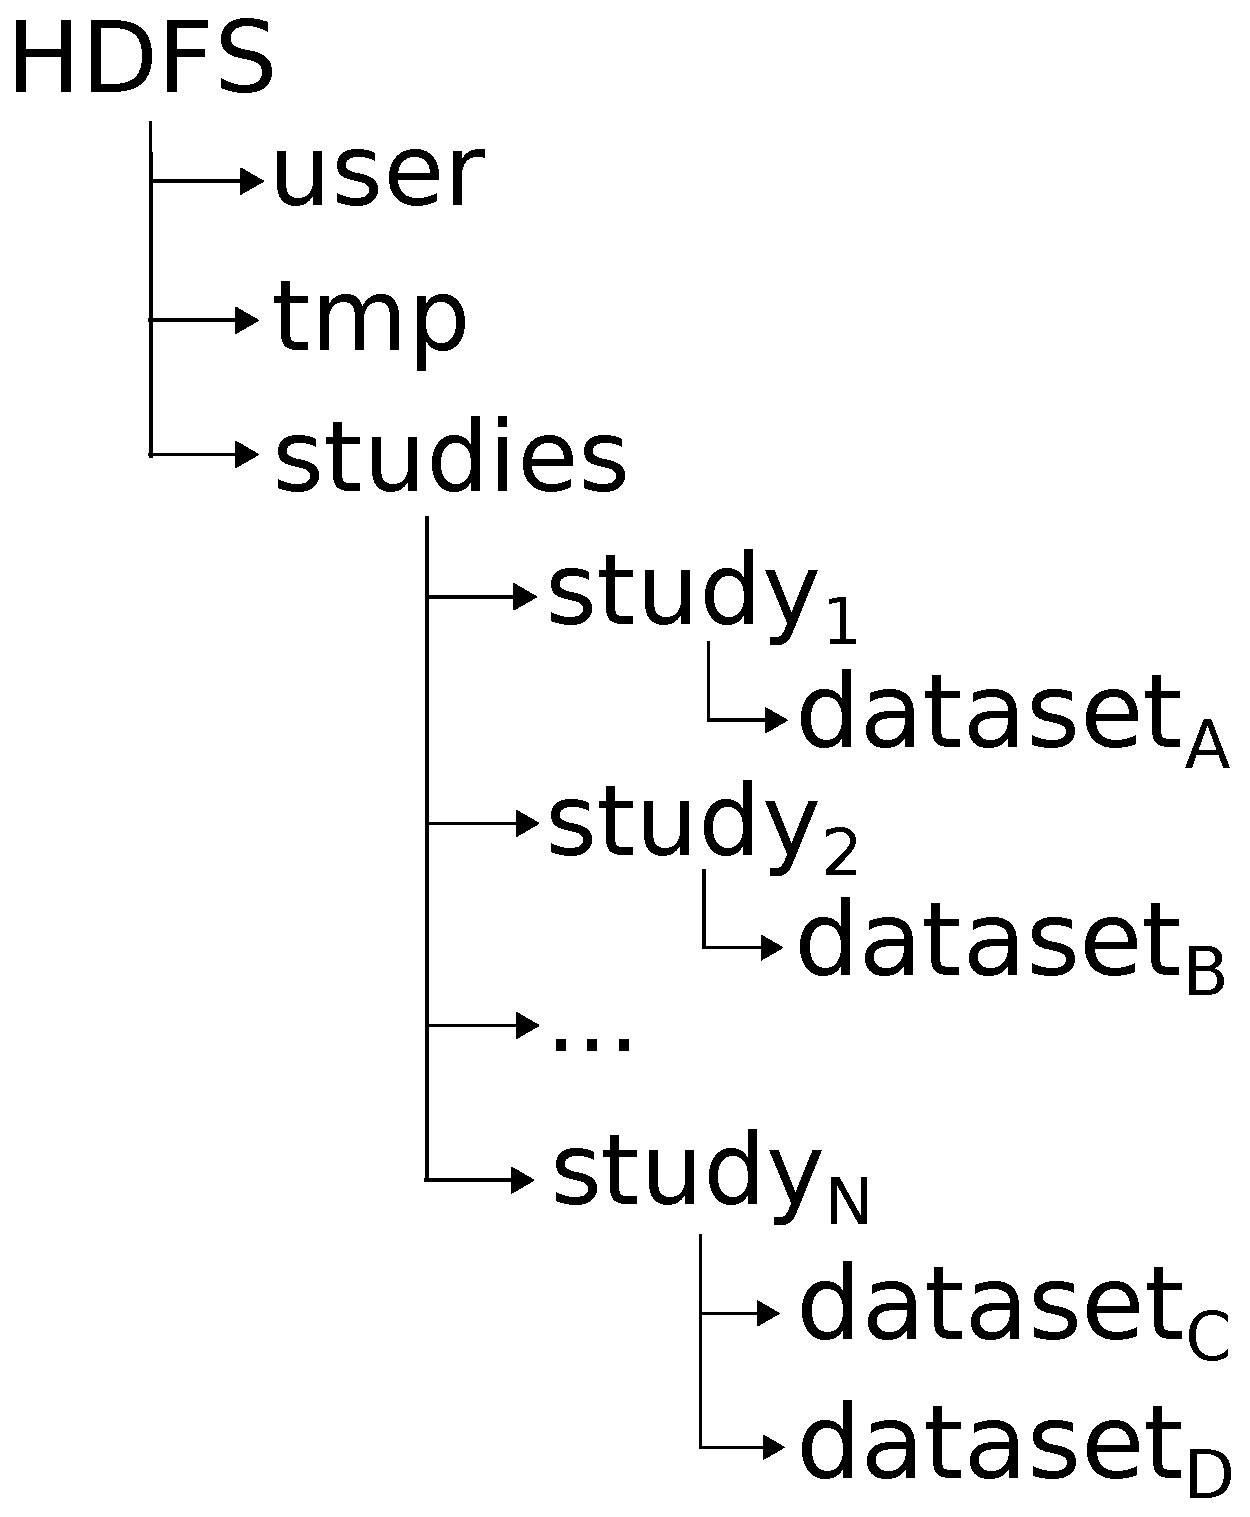
\includegraphics[scale=0.2]{./imgs/HDFS-structure.eps}
 % HDFS-structure.eps: 0x0 pixel, 300dpi, 0.00x0.00 cm, bb=0 -1 584 711
 \caption{Filesystem structure in HDFS containing Studies and DataSets.}
\end{figure}


\subsection {Auditing Service}
Finally, the auditing service enables the platform administrator or an external auditor to discover the history of accessing the platform to detect any violation to a policy. It includes several contexts \
such as role, account, study, and login audits. The secure login service assures that actions that are taken by the users are registered for tracing and auditing purposes. Each log event contains informat\
ion such as initiator, target, IP/MAC addresses, timestamp, action, and outcome.
